%!TEX root = ../main.tex

\chapter{Background}
\label{chp:background}

\section{DBMS and client GUIs}
\subsection{PostgreSQL}
\label{sec:postgres}
PostgreSQL, often called Postgres, is a robust open-source \ac{RDBMS} known for its flexibility, stability, and full compliance with SQL standards. It supports a wide range of advanced features, such as complex queries, foreign keys, views, triggers, and stored procedures. One of its distinguishing characteristics is its support for both structured and semi-structured data, including \ac{JSON}, making it suitable for modern applications that need to manage different data formats. PostgreSQL also offers powerful indexing techniques (e.g., B-tree, GIN, GiST) to optimize query performance, as well as Multi-Version Concurrency Control (MVCC), which enables high transaction throughput without locking issues, allowing multiple users to interact with the database simultaneously.

In the project developed at UNOX S.p.A., PostgreSQL is used to manage key operational data related to industrial ovens. This includes information about companies, devices (ovens), recipes, and device groupings. These datasets are critical for the \ac{DDC} platform, which leverages the stored information to enhance oven performance, improve operational processes, and provide customers with detailed insights.

PostgreSQL is considered a popular choice for many organizations since is open-source, has extensive community support, and is involved in continuous development. It offers a highly customizable solution for both small-scale applications and large enterprise systems.

\subsection{MongoDB}
MongoDB is an open-source NoSQL database designed to handle large volumes of unstructured and semi-structured data. Unlike traditional relational databases like PostgreSQL, described in the previous section \ref{sec:postgres}, which store data in structured tables with fixed schemas, MongoDB uses a flexible, document-based model. Data is stored in \ac{JSON}-like BSON (Binary \ac{JSON}) format, allowing for dynamic, schema-less storage where each document can have a different structure. This makes MongoDB ideal for use cases where data is heterogeneous or rapidly changing, as it does not require predefined schemas or rigid structures like a relational database.

In contrast to PostgreSQL, which excels at managing structured, relational data with well-defined relationships, MongoDB is optimized for handling data that doesn't fit into regular table structures, such as hierarchical or nested data. Additionally, MongoDB offers easy horizontal scaling, distributing data across multiple servers to handle high write loads, making it well-suited for applications that generate large amounts of real-time data.

At UNOX, MongoDB is used to store IoT data generated by the industrial ovens. This includes sensor readings like temperature, humidity, alarms, and detailed records of cooking processes. The flexible schema in MongoDB allows the system to efficiently capture and store a wide variety of data points, which may differ from oven to oven, or even from one cooking session to another. This dynamic approach enables real-time monitoring and analysis of oven performance, helping to ensure that the ovens operate efficiently and providing actionable insights based on the data collected.

\subsection{TablePlus}
TablePlus is a versatile database management tool designed to simplify working with relational databases. It supports a wide range of databases like PostgreSQL, MySQL, and SQLite, making it a go-to solution for developers who need to manage different database systems through a single interface. The most appreciated feature of TablePlus is its intuitive, streamlined interface, which enables users to easily run queries, edit data, and manage tables without needing to rely heavily on complex command-line tools.

The tool also emphasizes security, providing secure connections via SSH and SSL, which is crucial when dealing with sensitive data. It is lightweight and fast, ideal for those who require quick access to data and the ability to make changes efficiently. Other features that distinguish Table Plus among database professionals are the ability to preview and revert changes, multi-step undo, and export options enhance productivity, and reduce the risk of errors, making TablePlus a popular choice among database professionals.

\subsection{Studio 3T}
Studio 3T is a dedicated tool for managing MongoDB databases, offering a range of features designed to make interacting with NoSQL data easier. Unlike general database tools, Studio 3T is optimized for MongoDB's document-based structure. It provides a visual interface for building and executing queries, which is especially useful for those who prefer not to write complex MongoDB queries by hand.

Key features include the ability to migrate data, visualize aggregation pipelines, and easily manage indexes and collections. Studio 3T also allows users to translate \ac{SQL} queries into MongoDB's query language, making the transition for those familiar with \ac{SQL}-based databases smoother. It is a powerful tool for handling MongoDB-specific tasks, enabling developers and administrators to efficiently manage large datasets in a more user-friendly environment.

\subsection{Prisma}

\section{Amazon Web Services}
\acf{AWS} is a cloud computing platform that provides a broad set of services, including computing power, storage, and networking, through the internet. Businesses and developers use \ac{AWS} to build and run a wide variety of applications, from simple websites to complex enterprise systems. One of its key benefits is the ability to scale resources up or down based on demand, which eliminates the need for managing physical hardware and allows for greater flexibility. \ac{AWS} operates on a global network of data centers, offering services that ensure high availability and reliability for users across different regions. \ac{AWS} enables companies to access the resources they need with minimal upfront investment, through its modular services, such as \ac{EC2} for virtual servers and \ac{S3} for data storage. \ac{AWS} also promotes a pay-as-you-go pricing model, where users only pay for the resources they use, making it affordable for both small startups and large enterprises. Its extensive suite of tools allows users to implement everything from basic hosting solutions to advanced analytics and AI models.

Below, some of the \ac{AWS} tools used to build the system's architecture will be presented.
\subsection{IAM}
\ac{AWS} \ac{IAM} allows you to securely manage access and permissions to \ac{AWS} resources. With IAM, you can create and control users, groups and roles, assigning detailed permissions to specify who can access what resources and with what privileges. For example, you can grant a user access to certain \ac{AWS} services or specific actions on a database, while restricting other operations.

IAM uses the concept of "least privilege", allowing you to configure very precise accesses and monitor activities via logs. It is a fundamental tool for ensuring security and control in the \ac{AWS} infrastructure.
\subsection{Elastic Compute Cloud (EC2)}
Amazon \acf{EC2} is a main \ac{AWS} service that allows to launch and manage virtual servers in the cloud, called instances. \ac{EC2} offers a range of instance types to meet different computational needs, allowing users to select the optimal balance of CPU, memory, and storage for their workloads. Therefore, when you create an instance it is possibile to choose the specific hardware configurations that best suit their specific requirements, offering flexibility in performance and cost management. \ac{EC2} enables on-demand access to computing power, with the ability to deploy and manage instances without the need for physical servers.

\ac{EC2} also integrates well with other \ac{AWS} services, allowing to build reliable and scalable cloud-based systems. It supports multiple operating systems, such as Linux and Windows, and offers both temporary and persistent storage options, depending on the type of application.

For instance, in this project, an \ac{EC2} instance was used to host a snapshot of the production database, allowing safe testing and development with real data without affecting the live environment. This demonstrate how \ac{EC2} can help isolate and manage testing or development environments effectively.
\subsection{Relational Database Service (RDS)}
Amazon \ac{RDS} is an easy-to-manage relational database service optimized for total cost of ownership. It is easy to configure, use and scale according to demand. Amazon \ac{RDS} automates several database management tasks such as provisioning, configuration, backups and patching. Amazon \ac{RDS} allows customers to create a new database in some minutes and offers the flexibility to customize databases to their needs by choosing from 8 engines and 2 deployment options. Customers can optimize performance with features such as Multi-AZ with two readable standbys, optimized writes and reads, and \ac{AWS} Graviton3-based instances, with a choice of pricing options to manage costs effectively.

You have the option to enable automated backups or create manual backup snapshots as needed. These backups can be used to restore your database efficiently and reliably using Amazon \ac{RDS}'s restoration process.

Beyond the security features included in your database package, you can manage access by utilizing \ac{AWS} \ac{IAM} to assign user roles and permissions. You can also enhance database protection by placing them within a \ac{VPC}. Moreover, security groups can be used to control what IP addresses or Amazon \ac{EC2} instances can connect to your databases.


The table \ref{tab:ec2vsrds} compares the database management models between Amazon \ac{EC2} and Amazon \ac{RDS}, highlighting customer and \ac{AWS} responsibilities for various features.

\begin{table}[ht]
    \centering
    \begin{tabular}{|l|c|c|}
    \hline
    \textbf{Feature} & \textbf{\ac{EC2} management} & \textbf{\ac{RDS} management} \\ \hline
    Application optimization & Customer & Customer \\ \hline
    Scaling & Customer & AWS \\ \hline
    High availability & Customer & AWS \\ \hline
    Database backups & Customer & AWS \\ \hline
    Database software patching & Customer & AWS \\ \hline
    Database software install & Customer & AWS \\ \hline
    Operating system (OS) patching & Customer & AWS \\ \hline
    OS installation & Customer & AWS \\ \hline
    Server maintenance & AWS & AWS \\ \hline
    Hardware lifecycle & AWS & AWS \\ \hline
    Power, network, and cooling & AWS & AWS \\ \hline
    \end{tabular}
    \caption{Comparison of Amazon \ac{EC2} and Amazon \ac{RDS} database management models}
    \label{tab:ec2vsrds}
\end{table}

\subsection{Lambda}
\ac{AWS} Lambda is a serverless computing service that allows code to be executed without having to manage servers or infrastructure directly. Launched in 2014, Lambda allows developers to execute functions in response to specific events, such as changes to a database, \acused{HTTP}\ac{HTTP} requests, or file updates in an Amazon \ac{S3} bucket.

The serverless model eliminates the need for manual provisioning, management, or scaling of resources, as Lambda takes care of these tasks automatically. Users only pay for the code execution time, measured in milliseconds, and the number of requests, making it a highly cost-efficient option for many applications. The service supports several programming languages, including Python, Node.js, Java, Go, and C\#, making it flexible for a wide range of use cases, such as real-time data processing, application monitoring, and automation of repetitive tasks.

To generate a lambda, first, you create your function by uploading your code and choosing the memory, timeout period, and \ac{AWS} \ac{IAM} role. Then, you specify the \ac{AWS} resource to trigger the function, which can be a particular Amazon \ac{S3} bucket, Amazon DynamoDB table, or  Amazon Kinesis stream. When the resource changes, Lambda will run your function, launching and managing the compute resources as needed to keep up with incoming requests.
\subsection{Glue}\label{sec:glue}
\ac{AWS} Glue is a fully managed extraction, transformation and loading service, designed to facilitate the preparation and integration of data for analysis. \ac{AWS} Glue automates the processes of data discovery, cataloguing, cleaning, transformation and movement between different sources such as data lakes, relational databases and other storage resources. The service is designed to simplify the work of preparing data for analysis and modelling by eliminating the need to configure and manage servers. The three main features offered by Glue are:
\subsubsection{Jobs ETL}
\ac{ETL} Jobs in \ac{AWS} Glue are the main operating units that perform the extraction, transformation and loading processes. An \ac{ETL} job reads data from a source, transforms it as required (such as cleaning, merging or format conversion) and loads it into a destination, such as a data warehouse or data lake. \ac{AWS} Glue automatically generates Scala or Python code to perform these operations, but also offers the possibility of customising scripts. These jobs can be executed on demand or scheduled at regular intervals, integrating with other \ac{AWS} resources.
\subsubsection{Data Catalog}
The \ac{AWS} Glue Data Catalogue is a centralised metadata repository that organises and manages information on datasets from different sources. It stores data schemas, formats and partitions, facilitating access and queries via tools such as Amazon Athena and Amazon Redshift, without requiring manual configuration.
\subsubsection{Crawler}
\ac{AWS} Glue Crawlers automate data discovery and cataloguing by analysing sources to automatically identify schemas and partitions. They update or create tables in the data catalogue, reducing manual work and simplifying metadata management.

In summary, \ac{AWS} Glue, through the use of Jobs \ac{ETL}, Data Catalogue and Crawler, provides a powerful and scalable platform for large-scale data management, optimising workflows and ensuring easy integration with other \ac{AWS} services.
\subsection{Athena}
Amazon Athena is an interactive query service that allows data analysis directly on files stored in Amazon \ac{S3} using standard \ac{SQL}. Athena is a serverless solution, which means that it does not require the management of infrastructure or servers: users only pay for the queries executed, based on the volume of data processed.

The service is optimised to work with large datasets and common data formats such as \acused{CSV}\ac{CSV}, \ac{JSON}, Parquet and Apache ORC\footnote{\url{https://orc.apache.org/}}, Apache Iceberg\footnote{\url{https://iceberg.apache.org/}} allowing structured and semi-structured information to be analysed efficiently. Thanks to the \ac{AWS} Glue Data Catalogue described in the section \ref{sec:glue}, Athena can easily access previously defined metadata and schemas, reducing the time needed for data preparation.

Athena lends itself well to ad-hoc data lake analysis, reporting and data monitoring scenarios, without having to load data into a traditional database. Its features make it ideal for big data analytics environments, where speed of execution and ease of use are crucial, and it integrates well with other \ac{AWS} services, such as Amazon QuickSight for data visualisation.
\subsection{QuickSight}
Amazon QuickSight is a cloud-based \ac{BI} service from \ac{AWS}, designed to create dashboards, interactive visualisations and reports from large volumes of data. QuickSight empowers users to analyse data in a simple and intuitive way, providing tools to create charts, tables and advanced visualisations that help make data-driven decisions.
The tool supports two modes of data access:
\begin{itemize}
    \item SPICE (Super-fast, Parallel, In-memory Calculation Engine) mode, which uses an in-memory engine for fast analysis performance and is available for a fee,
    \item and Direct Query mode, which is free but generally slower, as it queries directly on data sources.
\end{itemize}
QuickSight allows dashboards to be shared with other users and offers support for access from mobile devices, making it a flexible tool for real-time data analysis and visualisation.

Finally, one of QuickSight's most innovative features is its integration with generative artificial intelligence, which allows analyses to be built quickly via natural language prompts. Users can enter simple questions or queries in natural language and get automatically generated charts, tables and insights. This makes the analysis of datasets more accessible even for those without technical expertise, speeding up the decision-making process.
\subsection{Step Functions}
\ac{AWS} Step Functions is a fully managed workflow orchestration service that allows different \ac{AWS} services to be coordinated in sequential or parallel workflows. Using \ac{AWS} Step Functions, complex processes can be defined as states, with each step in the workflow representing an activity, such as executing a job, waiting for an event or calling the API of any \ac{AWS} service, such as \ac{AWS} Lambda, Amazon \ac{S3} or \ac{AWS} Glue.

The service uses a visual representation based on a state machine model, allowing users to build and monitor workflows intuitively. Alternatively, workflows can be defined via \ac{ASL}, a \ac{JSON} language that allows the user to specify the behaviour of each state, conditions for passing between states, and error and exception handling criteria.

\ac{AWS} Step Functions is ideal for automating distributed processes such as data pipelines, application management and microservice orchestration. It also enables workflows with error handling, retries and conditional operations, ensuring process reliability and resilience. Its extensive support for long-running tasks make it a powerful tool for coordinating the execution of complex tasks in a secure manner.
\subsection{Event Bridge}
\ac{AWS} EventBridge is a fully managed event routing service, designed to connect applications using real-time event streams. It enables the creation of event-based architectures, where various services or applications automatically react to events generated by other \ac{AWS} applications or services. Each event represents an action or change of state, such as changes in a database or updates in an \ac{S3} bucket, and is routed to appropriate destinations according to predefined rules.

Specifically, the system built uses EventBridge Scheduler, a feature that allows events to be scheduled at regular intervals or at specific times. This service is useful for performing recurring tasks or planned actions, such as starting jobs on \ac{AWS} Lambda or other resources. In practice, the EventBridge Scheduler functions as a serverless 'cron', allowing time-based workflows to be automated without having to manage a dedicated infrastructure.
\section{File formats}
\subsection{Apache Parquet}
\label{sec:parquet}
Apache Parquet\footnote{\url{https://parquet.apache.org/}} is an open-source, column-oriented data file format designed for efficient data storage and retrieval. It provides high-performance compression and encoding schemes to manage complex datasets in bulk and is supported by many programming languages and analytics tools. Initially used exclusively in the Hadoop ecosystem, Parquet is now employed by platforms such as Apache Spark\footnote{\url{https://spark.apache.org/}} and various cloud services to meet the demands of data warehousing.

Parquet's main features include:
\begin{itemize}
    \item \textbf{Columnar storage}: Unlike row-based formats like \ac{CSV} or Avro, Parquet stores the values of each column next to one another, allowing for better compression and faster querying, especially when accessing only a subset of columns.
    \item \textbf{Self-describing}: Each Parquet file contains metadata, such as the schema and structure, facilitating interoperability between services that write, store, and read Parquet files.
    \item \textbf{Efficient compression}: By leveraging the fact that columnar data tends to be of the same type, Parquet achieves more effective compression than row-based formats. This reduces storage needs and accelerates data transfers.
    \item \textbf{Flexible encoding schemes}: Parquet supports various encoding schemes, such as Run-Length Encoding (RLE), Dictionary Encoding, and Delta Encoding, which further optimize compression and performance.
    \item \textbf{Schema evolution}: Parquet allows schemas to evolve over time by adding or removing fields without affecting existing data, making it ideal for dynamic environments.
\end{itemize}

\subsubsection{Row Format vs. Columnar Format}

\begin{figure}[H]
    \centering
    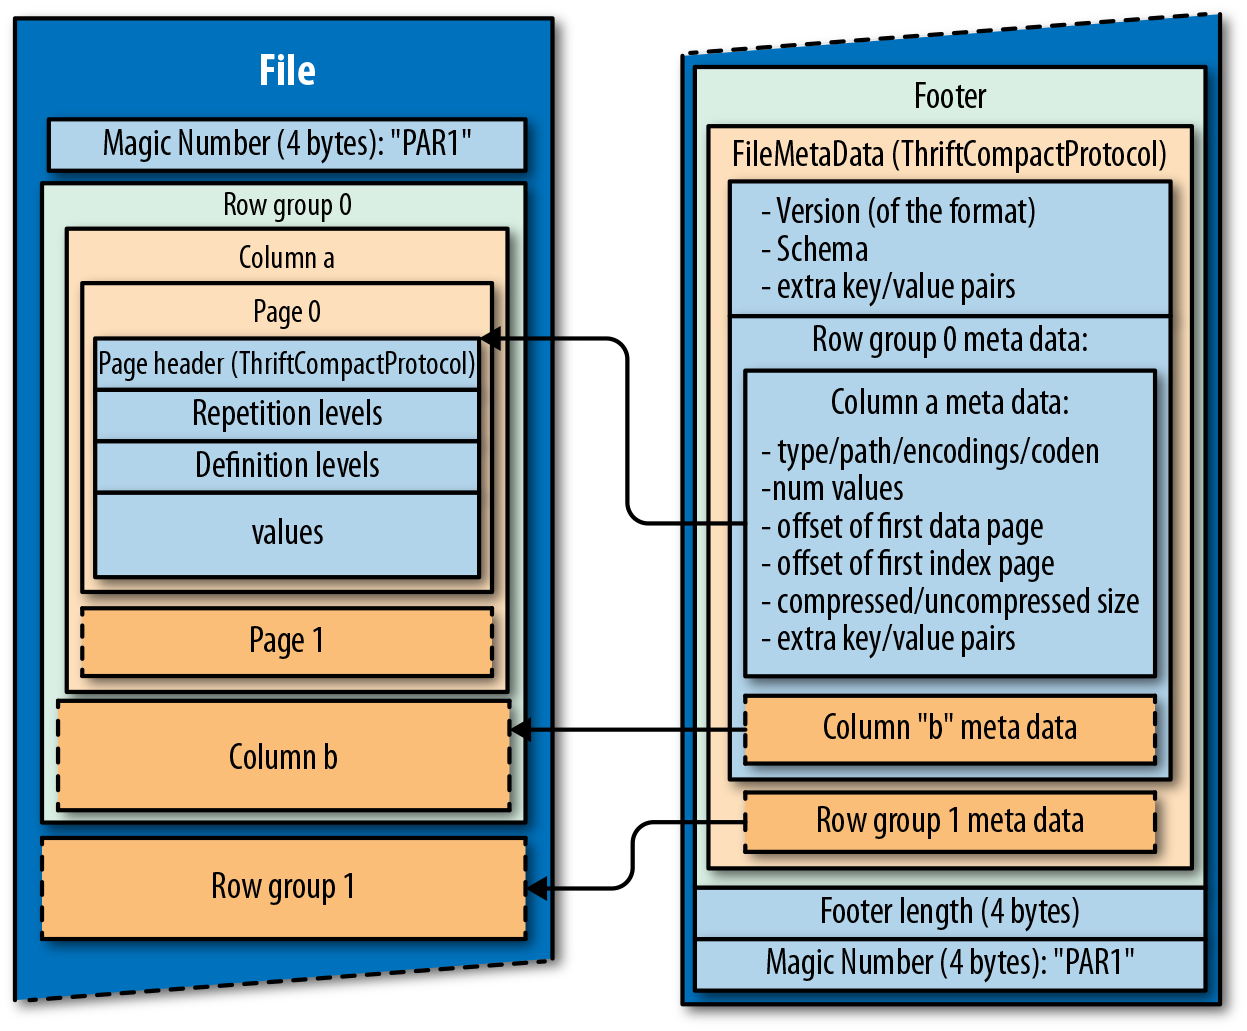
\includegraphics[width=0.7\textwidth]{res/ParquetFileLayout.png}
    \caption{Parquet File Layout}
    \label{fig:parquetlayout}
\end{figure}

As you can see in figure \ref{fig:parquetlayout}, each Parquet file contains a header, one or more data blocks, and a footer. The data itself is stored in the data blocks, while the footer holds metadata about row groups, columns, the Parquet format version, and a 4-byte magic number. The data is organized into:
\begin{enumerate}
    \item \textbf{Row groups}: These logically partition the dataset into rows. Each row group contains a column chunk for every column in the dataset. Row group size can be pre-configured: larger groups improve sequential I/O but need more buffer memory. A recommended size is between 512 MB and 1 GB.
    \item \textbf{Column chunks}: Each column chunk represents contiguous data for a specific column within a row group.
    \item \textbf{Pages}: A page is the smallest indivisible unit in Parquet, used for compression and encoding. The division into pages allows for more efficient compression and parallelized reads. Page size can be pre-configured:
    smaller data pages allow more precise reads, like single-row lookups, while larger pages reduce space and parsing overhead. The recommended page size is 8KB.
\end{enumerate}

This structure is optimized for analytical queries that only require a subset of columns, reducing I/O by reading less data. Moreover, Parquet files contain statistics like the minimum and maximum values for each column, enabling engines to skip irrelevant data blocks during queries.

\subsubsection{Compression Techniques}

In Parquet, compression is performed at the column level, supporting various encoding methods, including:
\begin{itemize}
    \item \textbf{Plain encoding}: The default encoding, used when no more efficient method is applicable.
    \item \textbf{Dictionary encoding}: Frequently occurring values are stored in a dictionary, and the data is replaced with the corresponding keys, reducing storage size. This method is applied dynamically when advantageous.
    \item \textbf{Run-Length Encoding (RLE)}: When consecutive values are the same, they are stored as a single value along with their count. Parquet combines bit-packing with RLE to achieve better compression.
    \item \textbf{Delta Encoding}: Instead of storing raw values, the difference between consecutive values is stored, which is useful for sequential data.
\end{itemize}

Parquet also supports compression algorithms such as Gzip, Snappy, Brotli, and LZO.

\subsubsection{Performance Benchmarking}

A benchmarking study conducted by Cloudera compares Parquet, Avro\footnote{\url{https://avro.apache.org/}}, and \ac{CSV} across various tasks \cite{parquet}. The results are summarized in Table \ref{table:parquetbenchmark}.

\begin{table}[h!]
    \centering
    \begin{tabular}{|l|l|l|l|}
    \hline
    \textbf{Metric}                 & \textbf{Parquet} & \textbf{Avro} & \textbf{CSV}  \\ \hline
    \multicolumn{4}{|c|}{\textbf{Narrow Dataset (3 columns, 83.8M rows)}} \\ \hline
    Dataset to file format (s)      & 74               & 72            & 45.33         \\ \hline
    Row count (s)                   & 5.33             & 5.33          & 45.33         \\ \hline
    Group by (s)                    & 9                & 24            & N/A           \\ \hline
    All data pass (s)               & 8.33             & 15.66         & N/A           \\ \hline
    Disk space (MB)                 & 750              & 1,000         & 4,000         \\ \hline
    \multicolumn{4}{|c|}{\textbf{Wide Dataset (103 columns, 694M rows)}}  \\ \hline
    Dataset to file format (s)      & 138              & 180           & 68            \\ \hline
    Row count (s)                   & 2.66             & 45.33         & 68            \\ \hline
    Group by (s)                    & 31               & 54            & N/A           \\ \hline
    All data pass (s)               & 33.33            & 140           & N/A           \\ \hline
    Disk space (GB)                 & 5                & 18            & 200           \\ \hline
    \end{tabular}
    \caption{Performance Comparison of Parquet, Avro, and \ac{CSV}}
    \label{table:parquetbenchmark}
\end{table}

From the table, it is evident that Parquet consistently outperforms Avro and \ac{CSV} in terms of storage space and query speed. For instance, Parquet files required only 750 MB of disk space for the narrow dataset, compared to Avro's 1 GB and \ac{CSV}'s 4 GB. Similarly, Parquet demonstrated a 97.5\% compression ratio on the wide dataset, allowing it to process 3.5 times less data in the same operations, compared to Avro. While Parquet performed well across the board, its efficiency is particularly notable for read-heavy operations, like analytical queries involving group-by and column scans.

Another study on the choice of the most efficient format in the Apache Hadoop system between parquet, orc, avro, \ac{CSV}, \ac{JSON} \cite{sym13020195} shows that Parquet is better than its competitors from the point of view of storage, all data search, unique row search and sorting. However, it has a similar performance to ORC in the grouping and filtering tasks.

However, Parquet can be slower to write than row-based formats like \ac{CSV} or Avro, due to the overhead of generating metadata.

\subsubsection{Use Cases and Limitations}

Parquet is particularly well-suited for scenarios that require efficient compression and fast query performance on large datasets.It is often used for analytical queries that need to access a subset of columns, in data pipelines where schema evolution is crucial, and in cases where efficient data storage and retrieval are key considerations.However, one limitation of Parquet is the potential performance drop when querying full rows in datasets with a very wide structure, typically with more than 100 columns. In such cases, row-based formats like Avro or ORC may offer better performance, as they are optimized for retrieving entire rows.

\subsection{Apache Iceberg}
Apache Iceberg\footnote{\url{https://iceberg.apache.org/}} is an open-source format for managing large tables in Data Lakes. Initially developed by Netflix and later open-sourced, Iceberg was designed to overcome the limitations of more traditional table formats such as Apache Hive, which do not scale well in complex and distributed Data Lakes. Iceberg natively supports table management on both Hadoop Distributed File System (HDFS) and cloud storage, such as Amazon \ac{S3}, Google Cloud Storage, or Microsoft Azure.

The primary goal of Iceberg is to provide a table format that efficiently supports the management of distributed data, allowing for reliable large-scale read and write operations, ensuring data consistency, and facilitating operations such as dataset scanning and version control.

Like Apache Parquet described in the previous section \ref{sec:parquet}, Iceberg is based on a layered architecture that separates metadata management from the data itself. This separate approach allows for more effective management of read and write operations and enables scalable modification operations. Metadata in Iceberg is crucial for table management. Iceberg uses a snapshot system to keep track of table versions, enabling rollback operations and ensuring full control of changes. The metadata includes information on schema, partitioning, data files, and delete files. Each data modification generates a new snapshot that can be consulted to view the table's evolution over time.

Since snapshots store details about the snapshot's timestamp, partition, and relevant data files, Iceberg supports versioning. Therefore, a snapshot provides a view of the entire dataset at a specific point in time.

\subsubsection{Iceberg Features}

Iceberg tables offer several benefits compared to other formats traditionally used in the data lake, including:

\begin{itemize}
    \item \textbf{Schema evolution}: Supports commands to add, drop, update, or rename columns without causing side effects or inconsistency.
    \item \textbf{Partitioning}: Iceberg introduces dynamic and flexible partitioning. Traditionally, Data Lakes use file path-based partitioning, which can be inefficient and difficult to manage. Instead, Iceberg implements a metadata-based partitioning strategy that reduces overhead and improves query performance. Two key improvements in partitioning are:
    \begin{itemize}
        \item \textit{Partition evolution}: Facilitates the modification of partition layouts in a table, such as data volume or query pattern changes, without needing to rewrite the entire table.
        \item \textit{Hidden partitioning}: Iceberg automatically handles partitioning by transforming column values (e.g., converting \texttt{event\_time} into \texttt{event\_date}) without requiring user-maintained partition columns. This allows queries to benefit from partitioning transparently, hiding the physical layout from producers and consumers. The separation of physical and logical partitioning enables the flexible evolution of partition schemes over time, improving performance without costly migrations.
    \end{itemize}
    \item \textbf{Time travel}: Allows users to query any previous version of the table to examine and compare data or reproduce results using past queries.
    \item \textbf{Version rollback}: Quickly fixes discovered issues by resetting tables to a known good state.
    \item \textbf{Increased performance}: Ensures data files are intelligently filtered for faster processing through advanced partition pruning and column-level statistics.
    \item \textbf{Transactional consistency}: Helps users avoid partial or uncommitted changes by tracking atomic transactions with \acused{ACID}\acs{ACID} (Atomicity, Consistency, Isolation, Durability) properties.
    \item \textbf{Table optimization}: Optimizes query performance to maximize the speed and efficiency with which data is retrieved. The main optimization is file compaction. This is particularly useful in Data Lakes, where data is often written in small files, causing fragmentation that can negatively impact query performance. Periodic compaction reduces the number of fragmented files and improves efficiency.
\end{itemize}

\subsubsection{ACID Operations}

One of the key contributions of Apache Iceberg to the Data Lake world is the implementation of support for \ac{ACID} operations, a crucial innovation to ensure the consistency and correctness of data operations.

\begin{itemize}
    \item \textbf{Atomicity}: Changes to the data are treated as atomic transactions, meaning multiple operations are applied as a block, ensuring they are either fully completed or not applied at all. This is particularly useful in scenarios requiring concurrent writes.
    \item \textbf{Consistency}: Thanks to advanced metadata management, Iceberg ensures that all operations on a table remain consistent, even in distributed environments.
    \item \textbf{Isolation}: Iceberg provides transaction isolation, ensuring that concurrent operations do not interfere with each other. Using a snapshot system, each read or write operation accesses a consistent version of the table.
\end{itemize}

These features make Iceberg ideal for managing highly reliable and resilient data pipelines.

\subsubsection{Table Layout}

The Iceberg table format offers similar capabilities to \ac{SQL} tables in traditional databases. However, unlike such datasets, Iceberg operates in an open and accessible manner, allowing multiple engines (such as Spark, Dremio\footnote{\url{https://www.dremio.com/}}, etc.) to work on the same dataset.

\begin{figure}[H]
    \centering
    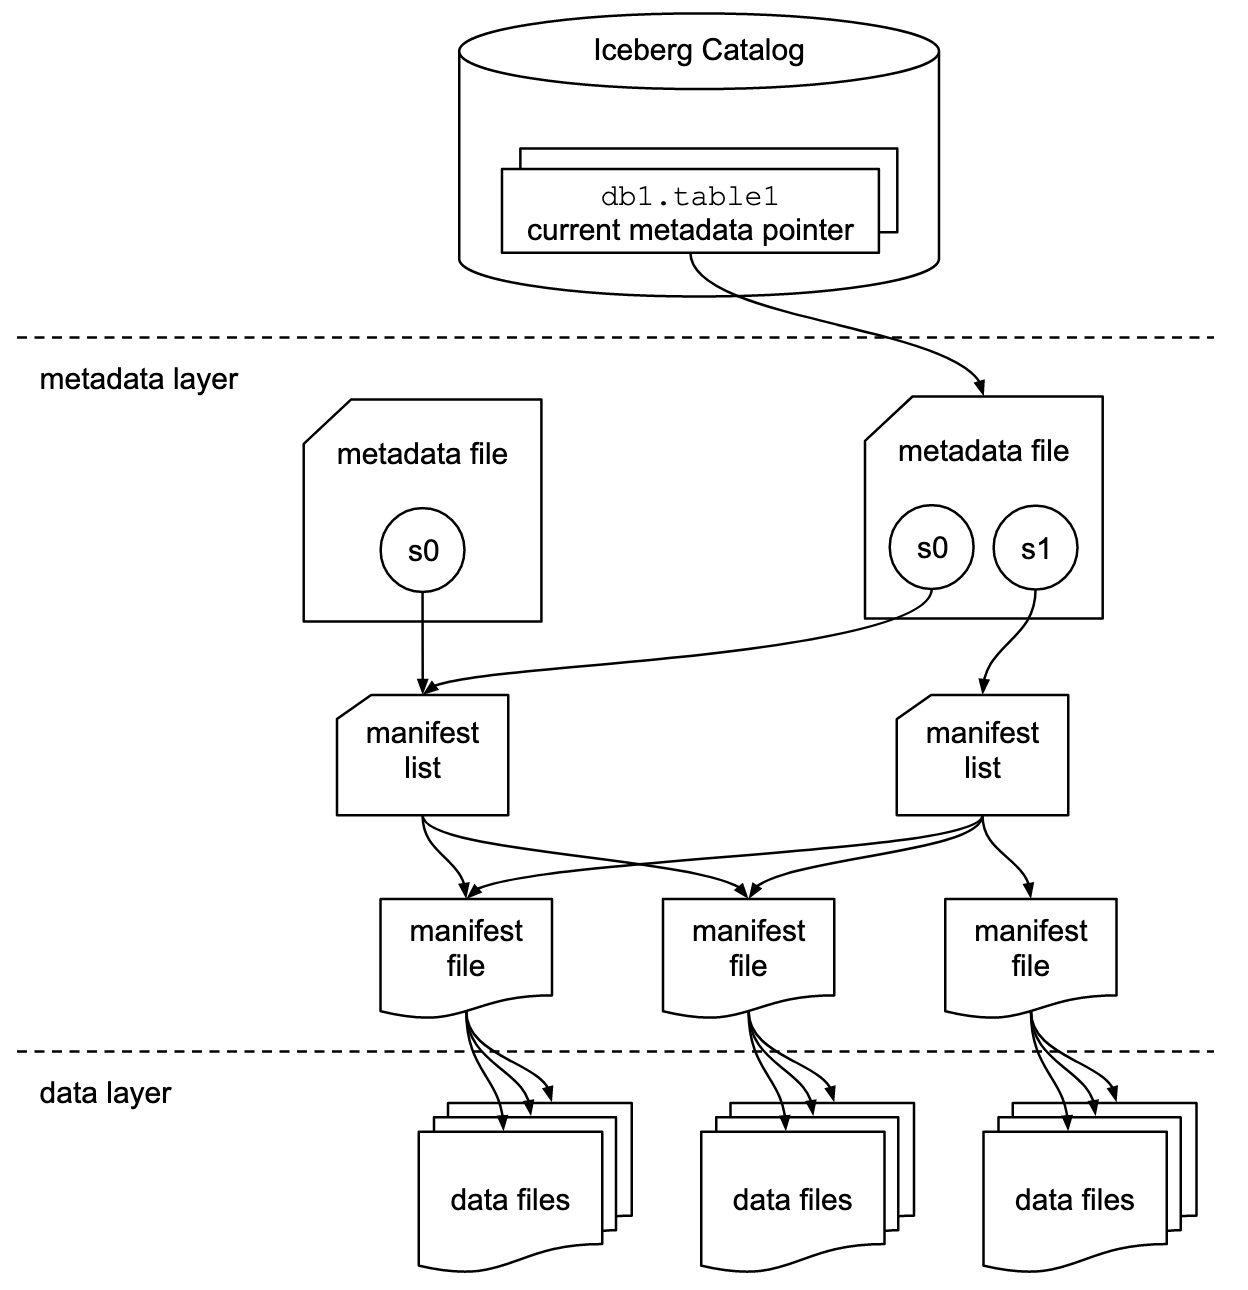
\includegraphics[width=0.7\textwidth]{res/IcebergFileLayout.png}
    \caption{Iceberg Table Layout}
    \label{fig:iceberglayout}
\end{figure}

Through metadata files, Iceberg tracks point-in-time snapshots by maintaining all deltas as a table. Each snapshot provides a full description of the table's schema, partition, and file information. Additionally, Iceberg intelligently organizes snapshot metadata hierarchically, enabling data processing engines to efficiently apply changes without redefining all dataset files, ensuring optimal performance at data lake scale.

The Iceberg table architecture consists of three layers:

\begin{itemize}
    \item \textbf{The Iceberg catalog}: This is where services find the location of the current metadata pointer, which helps identify where to read or write data for a given table. Each table's references or pointers exist here, identifying the current metadata file.
    \item \textbf{The metadata layer}: This layer consists of three components: the metadata file, the manifest list, and the manifest file. The metadata file contains information about a table's schema, partition details, snapshots, and the current snapshot. The manifest list includes a list of manifest files along with information about the manifests that form a snapshot. Manifest files track data files and include other details and statistics about each file.
    \item \textbf{The data layer}: Each manifest file tracks a subset of data files, which contain information about partition membership, record count, and column upper and lower bounds.
\end{itemize}